\documentclass[a4paper,12pt,twoside,abstraction,titlepage]{article}


\usepackage{verbatim}
\usepackage{latexsym}
\usepackage{exscale}
\usepackage{makeidx}
\usepackage{textcomp}
\usepackage{graphicx}
\usepackage{caption}
\usepackage{enumerate}
\usepackage{url}



\title{\Large \bf Implementation of Imputation Algorithm}
\author{Michelle Parker}

\linespread{1.18}

\begin{document}

\maketitle

\begin{abstract}
The aim of this document
\end{abstract}

\clearpage
\setcounter{tocdepth}{2}
\tableofcontents

 
\newpage

\section{Introduction}
The statistical definition of imputation is "a procedure for entering a value for a specific data item where the response is missing or unusable" \cite{unece}. In genetics, imputation refers to the process of inferring genotypes that are either missing, have a low quality score or are not directly assayed in sampled individuals.  This technique is used increasingly in genome-wide association and whole genome sequencing studies. 

Imputation has several uses: to boost power in a study by inferring erroneous, low confidence or sporadic missing data; to refine genotype probabilities; and to infer untyped data by using a reference panel containing a larger set of genetic markers.

In genome-wide association studies (GWAS), a number of genetic variants, usually single-nucleotide polymorphisms (SNPs), are assayed in groups of individuals with and without the disease of interest.  The selection of genetic variants used in the study are often genotyped using DNA microarrays; distinct types of microarray are composed of different selections of genetic variants across the genome.

Multi-marker association analysis, used in GWAS, identifies markers that are independently associated to the disease of interest.  Imputing sporadic missing data can make it easier to interpret the results of these analyses and can also boost power.  There may also be a number of genotype calling errors due low confidence data.  Imputation can be used to correct these errors which may help to control false-positive associations. \cite{review2009}.

A reference panel is a collection of samples genotyped at a dense set of markers across the genome.  These known haplotypes can be used to impute genetic variants that are not included on the SNP array used in the study.  This increases the number of SNPs that can be tested for association and advances fine-mapping studies where the location of the causal variant is identified. This technique can also be used in meta-analysis, where two or more studies conducted on different platforms are combined.  Stronger associations may be found with untyped SNPs than those that are genotyped even if the untyped SNP is poorly tagged, because imputation algorithms estimate haplotypes taking into account multiple markers surrounding the missing genotype \cite{review2010}.

The process of imputation is illustrated in Figure 1. Imputation is based on the identification of stretches of haplotypes which are shared between individuals.  These regions are known as being identical-by-descent (IBD) and would have originated from identical copies of the same ancestral allele.  Regions of IBD are much longer in closely related individuals than in unrelated individuals. In both related and unrelated samples, imputed haplotypes are modelled as mosaics of haplotypes in the reference panel.  When there is uncertainty over which haplotype is IBD, many imputation programs take this into account and summarize the information probabilistically.  Genotype likelihoods give a more accurate representation of the data and can often lead to more significant results when used in downstream analysis \cite{review2010}.

\begin{figure}[tp]
\begin{center}
\centerline{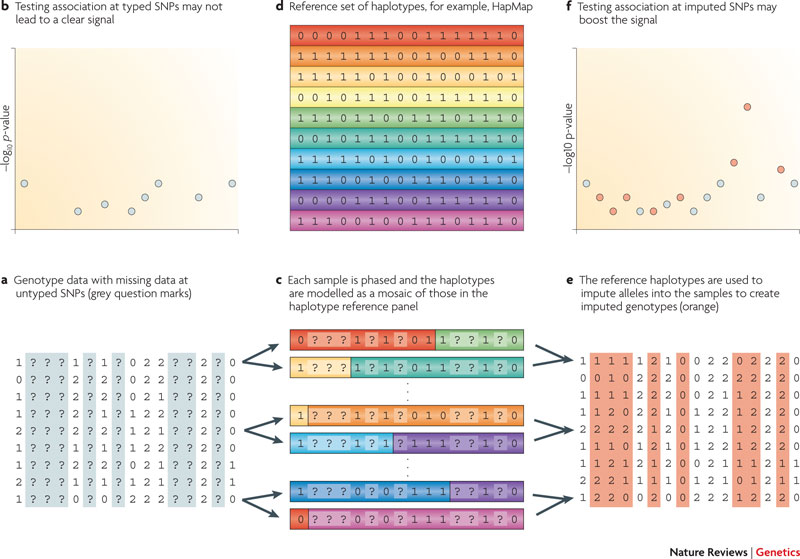
\includegraphics[scale=0.58]{reviewimage}}
\vspace{20pt}
\caption{This figure illustrates imputation of untyped SNPs in a sample of unrelated individuals using a reference panel \cite{review2010}.
\newline
Samples in the study are genotyped at a small number of sites using a microarray ({\bf a}). A reference panel ({\bf d}) of denser SNPs is used to infer the SNPs that have not been directly genotyped in the samples ({\bf c}).  In this process the samples are phased and the untyped SNPs are imputed ({\bf e}).
\newline
Testing association on just the SNPs which are directly assayed ({\bf a}) may not lead to a significant result ({\bf b}) but testing on all SNPs after imputation ({\bf e}), stronger associations on inferred SNPs may be found ({\bf f}).}
\end{center}
\vspace{-10pt}
\end{figure}

In low coverage whole genome sequencing, such as in the 1000 Genomes Project, imputation is used to assist genotype likelihood estimation and calling.  Relatively small amounts of sequence data across many individuals is combined to accurately estimate the genotypes for each sample.  In other words, the imputation algorithms use the sample data itself as its own reference panel \cite{1000genomes}.  Imputation can also be extended to include non-SNP variation such as copy number variation, classical human leukocyte antigen alleles, and short insertions and deletions (indels) \cite{review2010}.

There are many different methods for imputation based on different statistical models, but imputation algorithms can be divided into two main categories: those which take into account all observed genotypes during its computation of a single sample (IMPUTE, MACH, fastPHASE/BIMBAM), and those which only look at a window of markers either side of the missing genotype (BEAGLE, PLINK) \cite{review2009}.  Using all observed genotypes is computationally expensive but in many cases can achieve a more accurate result.  Factors which affect imputation accuracy include the size and choice of reference panel; the difference in genetic diversity between the study population and the reference panel; use of tagging methods for SNP array design.  In almost all cases, the larger the reference panel, the more accurate the imputation.  The algorithm implemented in this report uses a probabalistic graphical model and is described in the BEAGLE paper \cite{beagle3}.


\newpage
\section{Method}
The BEAGLE algorithm is structure in a similar way expectation-maximization (EM) algorithm.  An initial estimate of haplotype phase is obtained and then at each iteration, the model is fit and an improved estimate of haplotype phase is sampled.  The final output haplotypes are obtained by calculating the most likely based on the current model.

The process can therefore be split into 3 sections: model building, where a probabilistic graphical model is used to implicitely cluster haplotypes; sampling, where haplotypes are re-estimated and used as input into the next model build; and maximization, where the most likely haplotypes are extracted based on the current model.












\subsection{Model Building}




\subsection{Sampling}

\subsection{Maximization}


\subsection{Advantages of BEAGLE algorithm}

How beagle scales in number of samples and number of markers
Notes:
Why the beagle model is good

Does not need any prior informatino about haplotype frequency distribution. Models which require this type of estimation break down as the number of markers and samples increases because the number of observable haplotypes and the frequencies of these haplotypes become too small to estimate directly. If all feasible haplotypes are considered then this is very computationally expensive.
Other models include coalescent models which implies that haplotypes that are similar to the ones we have already seen are more likely to be seen again since changes in haplotypes occur thorugh recombination and mutation. Can produce very accurate results but can be computationally expensive as well
Other methods have made use of haplotype blocks but althorugh usefuly it does not adequately explain all the corelation struction between markers because LD can extend beyond block boundaries and can have more complex patterns within blocks
Automatically adapts to the amoung of linkage disequilibrium between markers.  No need to choose haplotype window size or select tagging markers.
Explain what linkage disequilibrium is - correlation structure between markers
Using a sliding window approach does not take into account how LD structure varies across the genome or areas where LD does not exist due to recombination hotspots 
Clusters haplotypes to improve power.


How beagle works

Localized haplotype-cluster model is an empirical LD model that adapts to the local structure in the daata. Relative to other methods it does well with large data sets. This methods can essentially be thought of as similar to an EM approach where and initial guess athaplotype phase is made, the model is fit, improved estimates of the haplotype phaseis made and the model is refit etc

\newpage
\section{Implementation}

\newpage
\section{Testing and Results}


\newpage
\section{Future work}

\newpage


\begin{thebibliography}{99}

\bibitem{unece} Economic Commission for Europe of the United Nations (UNECE), \emph{Glossary of Terms on Statistical Data Editing}, Conference of European Statisticians Methodological Material, Geneva. 2000

\bibitem{review2009} Yun Li, Cristen WIller, Serena Sanna \& Goncalo Abecasis, \emph{Genotype Imputation}, Annual Review of Genomics and Human Genetics, Volume 10, Issue 1,  2009, Pages 387-406

\bibitem{review2010} Jonathan Marchini \& Bryan Howie, \emph{Genotype Imputation for Genome-Wide Association Studies}, Nature Reviews Genetics, Volume 11, Issue 7, July 2010, Pages 299-511

\bibitem{1000genomes} 1000 Genomes Project Consortium, \emph{An integrated map of genetic variation from 1,092 human genomes}, Nature, Volume 491, Issue 7422, October 2012, Pages 56-65

\bibitem{beagle3} Sharon R. Browning \& L. Brian Browning, \emph{Rapid and Accurate Haplotype Phasing and MIssing-Data Inference for Whole-Genome Association Studies By Use of Localized Haplotype Clustering}, The American Journal of Human Genetics, Volume 81, Issue 5, November 2007, Pages 1084-1097

\bibitem{beagle1} Sharon R. Browning, \emph{Multilocus Association Mapping Using Variable-Length Markov Chains}, The American Journal of Human Genetics, Volume 78, Issue 6, June 2006, Pages 903-913



\end{thebibliography}

\end{document}  

